\documentclass[twoside,a4paper,12pt]{article}
\usepackage[applemac]{inputenc}
\usepackage{wrapfig}
\usepackage{graphicx}
\usepackage{graphics}
%\usepackage{subfig}
%\usepackage{inputenc}
\usepackage{amsmath}
\usepackage{amsfonts}
\usepackage{amssymb}
\usepackage[singlelinecheck=false]{caption}
\usepackage{array}
\usepackage{multirow}
\usepackage{setspace}
\usepackage{hyperref}
\usepackage{verbatim}
\usepackage[clearempty]{titlesec}
\usepackage{epstopdf}
\usepackage{lineno}
\usepackage{textcomp}
\usepackage{nicefrac}
\usepackage{xspace}
\usepackage{todonotes}
%\usepackage{autoref}
\usepackage[small, bf, hang, raggedright]{subfigure}

\usepackage[english]{babel} 

\onehalfspacing
\usepackage[left=2.9cm,right=2.9cm,top=3cm,bottom=4.5cm]{geometry}
\newcommand\leerseite{\newpage\thispagestyle{empty}\hspace{1cm}\newpage}

\newcommand{\subfigureautorefname}{\figurename}

\newcommand\piminus{\(\mathrm{\pi^-}\)}
\newcommand\muminus{\(\mathrm{\mu^-}\)}
\newcommand\eminus{\(\mathrm{e^-}\)}
\newcommand\eplus{\(\mathrm{e^+}\)}
\newcommand\geant{\textsc{Geant\,4}\xspace}

\begin{document}\selectlanguage{english}




\section*{Answers to Djamel's comments from 24.03.2016}
Dear Djamel,

Thank you for comments on my CAN draft. Please find my answers between your quotes below:

\begin{quote}\texttt{- A general remark:
At some stages of the analysis, it is mentioned that low energy pions have different behaviour compared to high energy pions. To have an overall picture of the detector response we used to scan its response to a wide energy range of pions which allows to be sensitive to various properties (noise, stat terms, etc), low energies being the most difficult to study because of the beam conditions.
But because PFA jets will deal with hadrons which are typically <10GeV I would suggest not to make the reader (or listner) think that low energies are a weak point. This is true for all the test beam studies I see on HCALs!}\end{quote}
I agree in principle. However except for the comment around line 268 about the 4\,GeV energy point preferring slightly different standard reconstruction weights than the other energies (in both data and MC) all remarks of that kind do directly reference the beam quality as the underlying issue I believe. Do you have any specific sentences in mind that you would propose to adjust? 

\begin{quote}\texttt{- line \#17: "... granularity requirements"
It is true however this is not the only property of these calorimeters. For example, an ECAL with a good granularity and a too large Moliere Radius leads to bad performances in terms of PFA.}\end{quote}
I generalised the sentence for the next draft.

\begin{quote}\texttt{- line \#16: "... as hadrons [..] PFS performances."
It is true. However one could say that this is of secondary importance compared to the capability to separate changed hadrons from neutral hadrons. The latest being the only component of the jet which relies on the intrinsic HCAL energy resolution. The way it is written sounds like the energy contribution of all the hadrons is measured with HCAL. PFA will use the tracker for the charged ones.}\end{quote}
I agree my use of ``hadrons'' was slightly misleading. What I meant is that we are interested in the single pion performance of our prototypes as it is the best measure of the general performance of the system as long as no full PFA system including a tracker and surrounding magnetic field is available. I altered the sentence accordingly for the next draft. 

\begin{quote}\texttt{- Table \#1: is the variation of the efficiency versus beam energy?
It seems from Table A4 you see the same shape on simulation so this not only due to beam conditions. Do you have an explanation?}\end{quote}
Calling the fraction of selected events ``efficiency'' on beam data is problematic, since the actual number of pions in the data sample is not known. I have thus changed ``Efficiency'' to ``$\frac{\text{Events (sel.)}}{\text{Events (raw)}}$''.

The fraction of selected events being much smaller at 4\,GeV is due to the combination of beam conditions and a different mode of operation of the differential Cherenkov counter. 

For Energies $\geq$12\,GeV the Cherenkov pressure is configured to do both pion tagging on one channel and electron rejection on the other channel. The pion tag was fed into the online trigger decision, while the electron rejection is recorded with the data and can be used in the offline analysis. We discovered that the Cherenkov-based electron rejection is also rejecting lots of pions, thus we do not use it in the offline event selection. Electron rejection is suitably done by the minimum FHI layer requirement (see also answer to next question).

For the 4\,GeV energy point, the Cherenkov gas pressure could not be increased high enough for an effective pion tag, and thus the pion tag ist not used in the online trigger decision. This gives a much higher fraction of electrons in the recorded 4\,GeV data (anyway the electron fraction in the beam is higher at 4\,GeV than at the other energies) and thus a smaller selected event fraction. Additionally there is an inefficiency in the FHI layer cut at 4\,GeV, see answer to next question. 

The ``shape'' on the efficiencies in table A.4 is due to different selection efficiencies of the multi particle suppression for single pion events. It seems that the efficiency of this cut goes down with increasing beam energy. Still there is no significant bias on response or resolution from this (in MC) as shown in the same table.

\begin{quote}\texttt{- line \#192: about FHI layer>=5
Does it create an inefficiency at low pion energies ?}\end{quote}
Yes it does, but not because of the general diffeerence between the FHI layer spectra of 4\,GeV pions and 32\,GeV, see \autoref{fig:fhi_truth} (sorry for the ugly quick and dirty plot). Instead this is due to the reduced accuracy of the reconstructed FHI layer at 4\,GeV compared to higher beam energies.
\begin{figure}[htbp]
\begin{center}
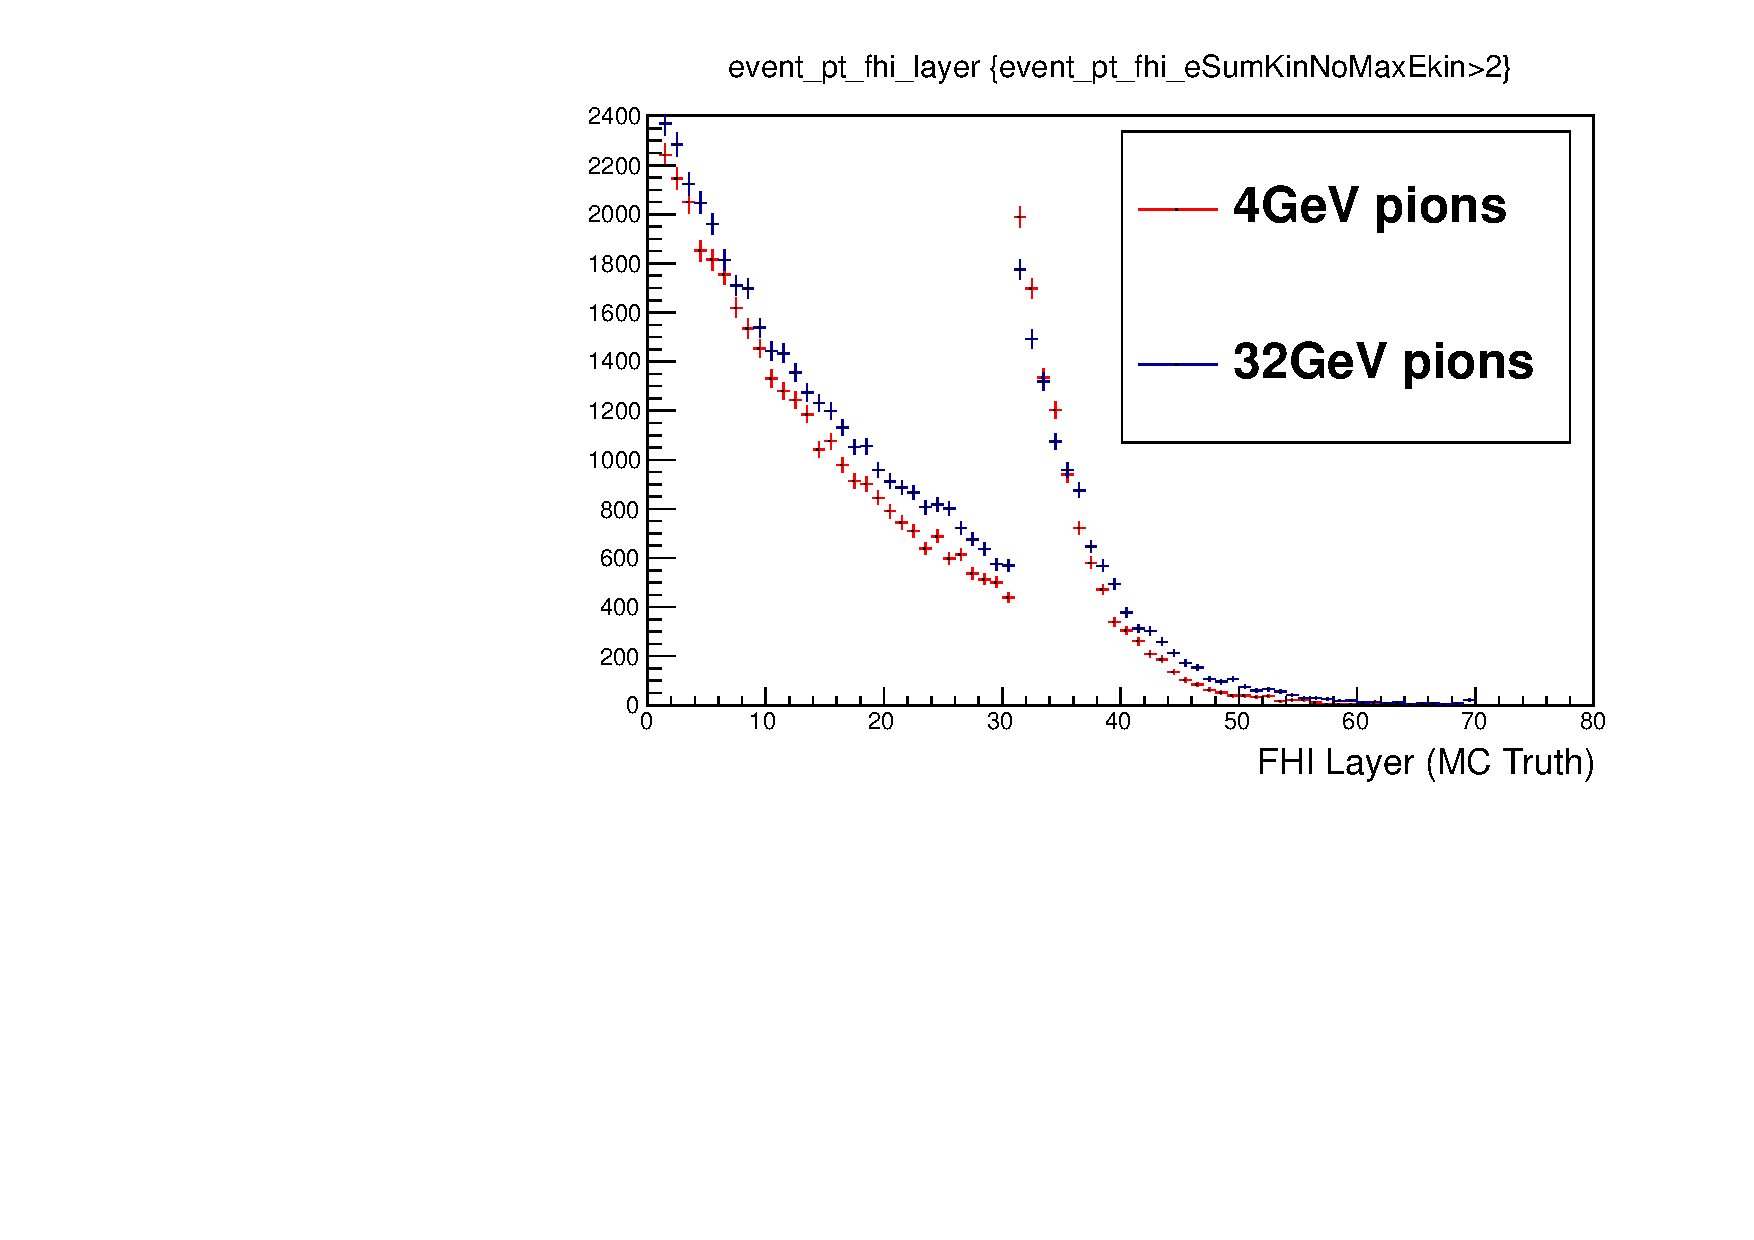
\includegraphics[width=0.8\textwidth,page=1]{fhi_truth_4gev_32gev}
\caption{MC truth distribution of FHI layer for 4\,GeV and 32\,GeV pions.}
\label{fig:fhi_truth}
\end{center}
\end{figure}

\begin{quote}\texttt{- line \#247: to avoid any biais you take the same number of events per beam energy.
Isn't it anyway biased by the available beam energies ?
eg. if you had 4, 19,20,21, 50 GeV pion data, keeping the same number of events at each energy points would give more weight to 20 GeV. I would instead keep the same statistics per energy bins. 4, 19-21, 50 in my example.
I don't think this would change significantly your results but is related to the general remark.}\end{quote}
I agree. However I do not see how the available beam energies (4\,GeV, 12\,GeV, 15\,GeV, 20\,GeV, 32\,GeV) should be binned, except for maybe putting 12\,GeV and 15\,GeV into one bin. In this case the linearity and resolution (see answer to next question) would get worse for these points (as they have less weight), however 12\,GeV already is the worst linearity energy point we see (interestingly in both data and MC).


\begin{quote}\texttt{- Eq 1: Such a Chi2 doesn't make any difference between non linearity and resolution. Did you try to use a Chi2 from which the reconstructed mean value is subtracted (based on spread only) and treat the linearity separately (based on mean only) ?
This could take time so if it was not tried already could you please estimate from what you have seen if it makes sense?}\end{quote}
I believe it is fundamentally flawed to treat linearity and resolution separately. In the special case of the standard reconstruction this would be possible when optimising each run by itself, as there are two variables (ecal and hcal weight) and two observables (response and resolution). In this case one could first optimise the ideal (in terms of relative width of the distribution) scaling ratio between ecal and hcal weight and then scale both parameters so that the mean reconstructed energy is exactly at the beam energy. However this would definitely lead to slightly different ideal weights for each beam energy. The whole point of the standard energy reconstruction is to be independent of beam energy (to be able to use the standard reconstructed energy as an estimate for more sophisticated algorithms like the software compensation described in the note).

In any other case with more parameters, optimising for ideal resolution while neglecting linearity will lead to absurd edge case results. To quote Felix: ``A single Geiger counter has perfect energy resolution, but miserable linearity''. I do not have an idea how one would go about optimising resolution and linearity sequentially.

\begin{quote}\texttt{- line \#274: ".. thus not notably influence resolution .."
This is true at particle level but an energy dependent bias at particle level leads to a degradation of PFA-jet resolution (sum of several non consistent biases leads to a spread).}\end{quote}
The bias is not energy dependent. It's a constant $\approx5\%$ deposition shift in MC for all energies and physics lists, see also the comparison of the ecal/hcal weight ratios in data and MC in Fig.7 (squares) is exactly identical in data and MC.

\begin{quote}\texttt{- Figure \#7:
You will apply on 4GeV pions slightly non optimal weights by ~8\% in AHCAL+TCMT (optimal value being governed by >10GeV pions).
Do you know if the a non optimal weight applied to 4GeV pions leads to an energy distribution larger than what it could have been with 4 GeV dedicated weights or to a shifted energy distribution ? (as mentioned before the Chi2 will not distinguish non-linearity from a bad resolution)}\end{quote}
The standard weights optimised for all runs give a mean response of 3.98\,GeV with 23.4\% resolution. Applying the standard weights optimised for the 4\,GeV point gives a mean response of 3.87\,GeV with 23.1\% resolution.

\begin{quote}\texttt{- line \#312:
You describe how you weight/count the hits. 
For my curiosity: did you test different configurations before reaching the optimal one?}\end{quote}
Not in great detail. From the SDHCAL reconstruction we know that counting hits can have positive effects due to suppression of Landau fluctuations. The central limit theorem tells us that when adding up multiple Landau-fluctuating hits the sum will again be somehow more similar to a Gaussian. We tried all bins weighted (no bins counting) first, then saw a small improvement in overall resolution when using the first two bins counting (as it is now) and then a very minimal, barely significant, decrease in overall resolution when going to only the first bin counting. The general effect of the counting bins is very small. I already proposed to change the whole analysis to only the first bin counting, what do you think about that?

\begin{quote}\texttt{- line \#322:
Hits from primary track are excluded. I sounds reasonable and I understand why.
For my curiosity, did you see if the number of layer (track length) depends on energy, like a logarithmic dependence ?}\end{quote}
Do you mean the mean primary track length as a function of particle energy? The influence of particle energy on the FHI layer spectrum is very small (see \autoref{fig:fhi_truth}), so there is barely any influence on the mean track length in the energy range examined here. This can also be seen from Fig12.(a) and (c), the first (track) bin is identical for both energies.

\begin{quote}\texttt{- Eq 3 and line \#299:
I probably misunderstood something as I do not see what rho from line \#299 corresponds to.
In general what are the 51 parameters you mentioned?}\end{quote}
I tried to explain this at the end of the same sentence. Do you have an idea how to modify this sentence to make this clearer?

The 51 parameters are from 8 hit energy bins in the ecal, parametrised with 3 parameters (2nd order polynomial) each, plus the same in the AHCAL, plus three parameters for the TCMT. 8*3+8*3+1*3 = 51. 

\begin{quote}\texttt{- line \#335:
Is this optimisation performed in the same way as for the standard reco method?}\end{quote}
In general yes, the optimisation $\chi^2$ function and general procedure is identical (a clarifying sentence about this was added to draft v1.2). Or do you mean the usage of the known beamenergy as $E_\text{est}$? This is not needed in the standard reconstruction optimisation, as the standard reconstruction does not depend on the beam energy.

\begin{quote}\texttt{- Figure 15.c:
Do you understand the shape which is similar in data and simulation? It seems correlated to the selection efficiency of Table 1.}\end{quote}
I assume you mean the deviation from linearity plots in Fig.15 and especially why the 12\,GeV point deviates by -2\% for data and all MCs?
Jerry asked a very similar question, so I quote my response to him (this also relates to one of your earlier questions about biasing of the optimisation from distribution of runs in beam energy):

``I do not know for sure. There is no statistical bias between runs, as each run is using the same number of events (40k in data, 20k in MC) for optimising the weights. However there is some inherent biasing because of the distribution of runs in energy (assume we would have runs at 1, 2, 3, 4, and 32\,GeV, even when using the same statistics in each run the 32\,GeV run would probably reconstruct worse as the optimisation will favor the lower energy par). Assuming that hadronic interactions show a different behaviour at 4\,GeV and 12+\,GeV (e.g. in MC the mean number of secondary particles produced in the first inelastic hadronic interaction is much higher at 4\,GeV than at 12\,GeV and upwards! I don't know if this is also seen in real life or just an effect of switching between different parametrisations in MC in that energy range though), the fact that there is no energy points in between 4\,GeV and 12\,GeV somehow causes a hard transistion. There are not enough degrees of freedom in the parametrisation (every weight is a 2nd order polynomial as a function of the beam/reconstructed energy) for a hard step, so the optimisation optimises the overall $\chi^2$. As the behaviour is the same in data and MC (at least in the SC case) I do not believe the dataset is compromised.''

\begin{quote}\texttt{- Comparison of data/MC weights:
You describe some weight differences between data and simulation.
They are determined by an optimisation process, so they represent the weights which minimise the overall distance between events and beam energies. Any phenomena which create a spread or a bias affect the weight values. Could it be due to beam conditions which can be quite different from a run to another one?}\end{quote}
I agree. We have reason to believe there is around 1\% (see my answer to Jerry on the INDICO page for details about estimated biases from that on resolution and response) remaining contaminated events after the pion selection. To minimise the effects on the parameter optimisation as far as possible (which can be influenced badly by single outlier events due to the square-distance weighting in the $\chi^2$) only the central 90\% standard reconstructed energy events are used for the parameter optimisation. There might of course still be an influence from contaminated events, but it should be minimal and I do not believe it is enough to cause the observed differences in weight.

I also added some text and two plots as Fig17 of the latest draft v1.2 (on INDICO) showing what happens when the data samples are reconstructed using the software compensation weights from MC. Interestingly the resolution very slightly improves over the MC, but the linearity becomes slightly worse.

I will reread my current draft for typos and upload it to INDICO in the next days.

Thank you again and cheers,
Oskar

\end{document}
